\chapter{程式碼}\

\section{球員控制程式}
 
 \begin{figure}[hbt!]
\begin{center}
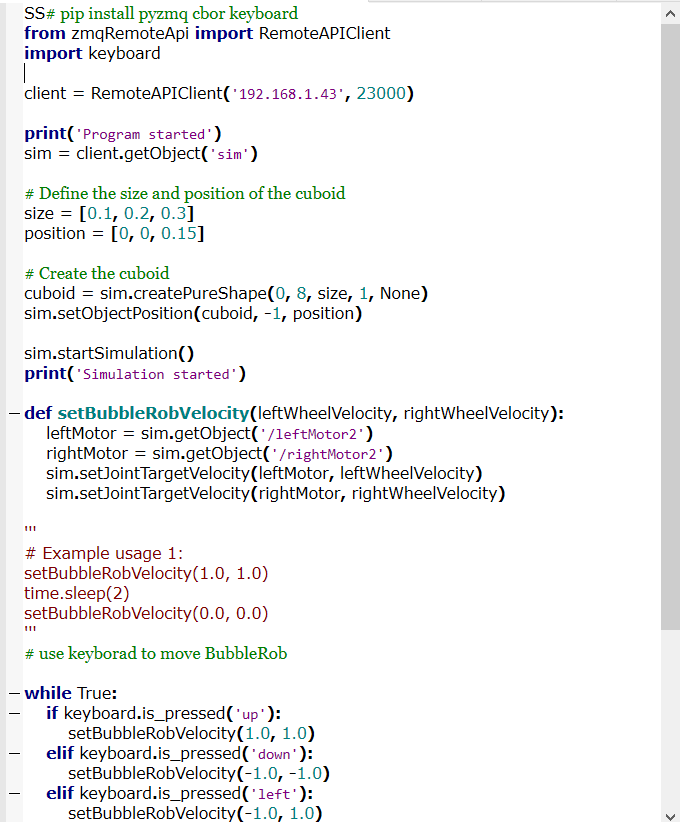
\includegraphics[width=10cm]{程式碼1}
\caption{\Large 球員控制程式碼}\label{fig.程式碼1}
\end{center}
\end{figure}

\begin{center}
 使用 RemoteAPIClient 來連接遠端的 API 服務器,以及使用keyboard 函式庫來控制鍵盤。\\
 \end{center}
 
\begin{figure}[hbt!]
\begin{center}
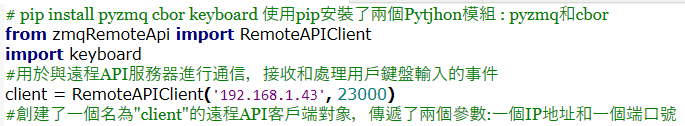
\includegraphics[width=13cm]{程式碼2}
\caption{\Large RemoteAPIClient}\label{fig.程式碼2}
\end{center}
\end{figure}

\newpage
 
\section{連線程序}

\begin{center}
主機的部分要先到小黑窗打指令ipconfig,搜尋本機位址
\end{center}

\begin{figure}[hbt!]
\begin{center}
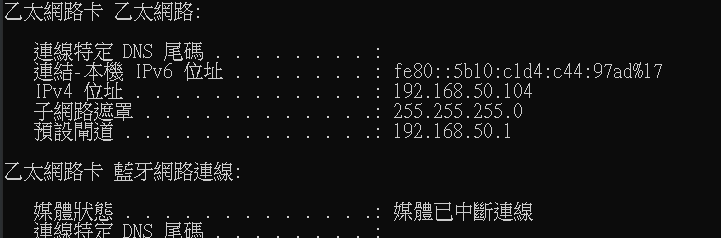
\includegraphics[width=12cm]{程式碼6}
\caption{\Large 查詢網路位址}\label{fig.程式碼6}
\end{center}
\end{figure}

\begin{center}
為了能在操控球員時能夠實時看到球場上的情況,所要做的前置作業
\end{center}

\begin{figure}[hbt!]
\begin{center}
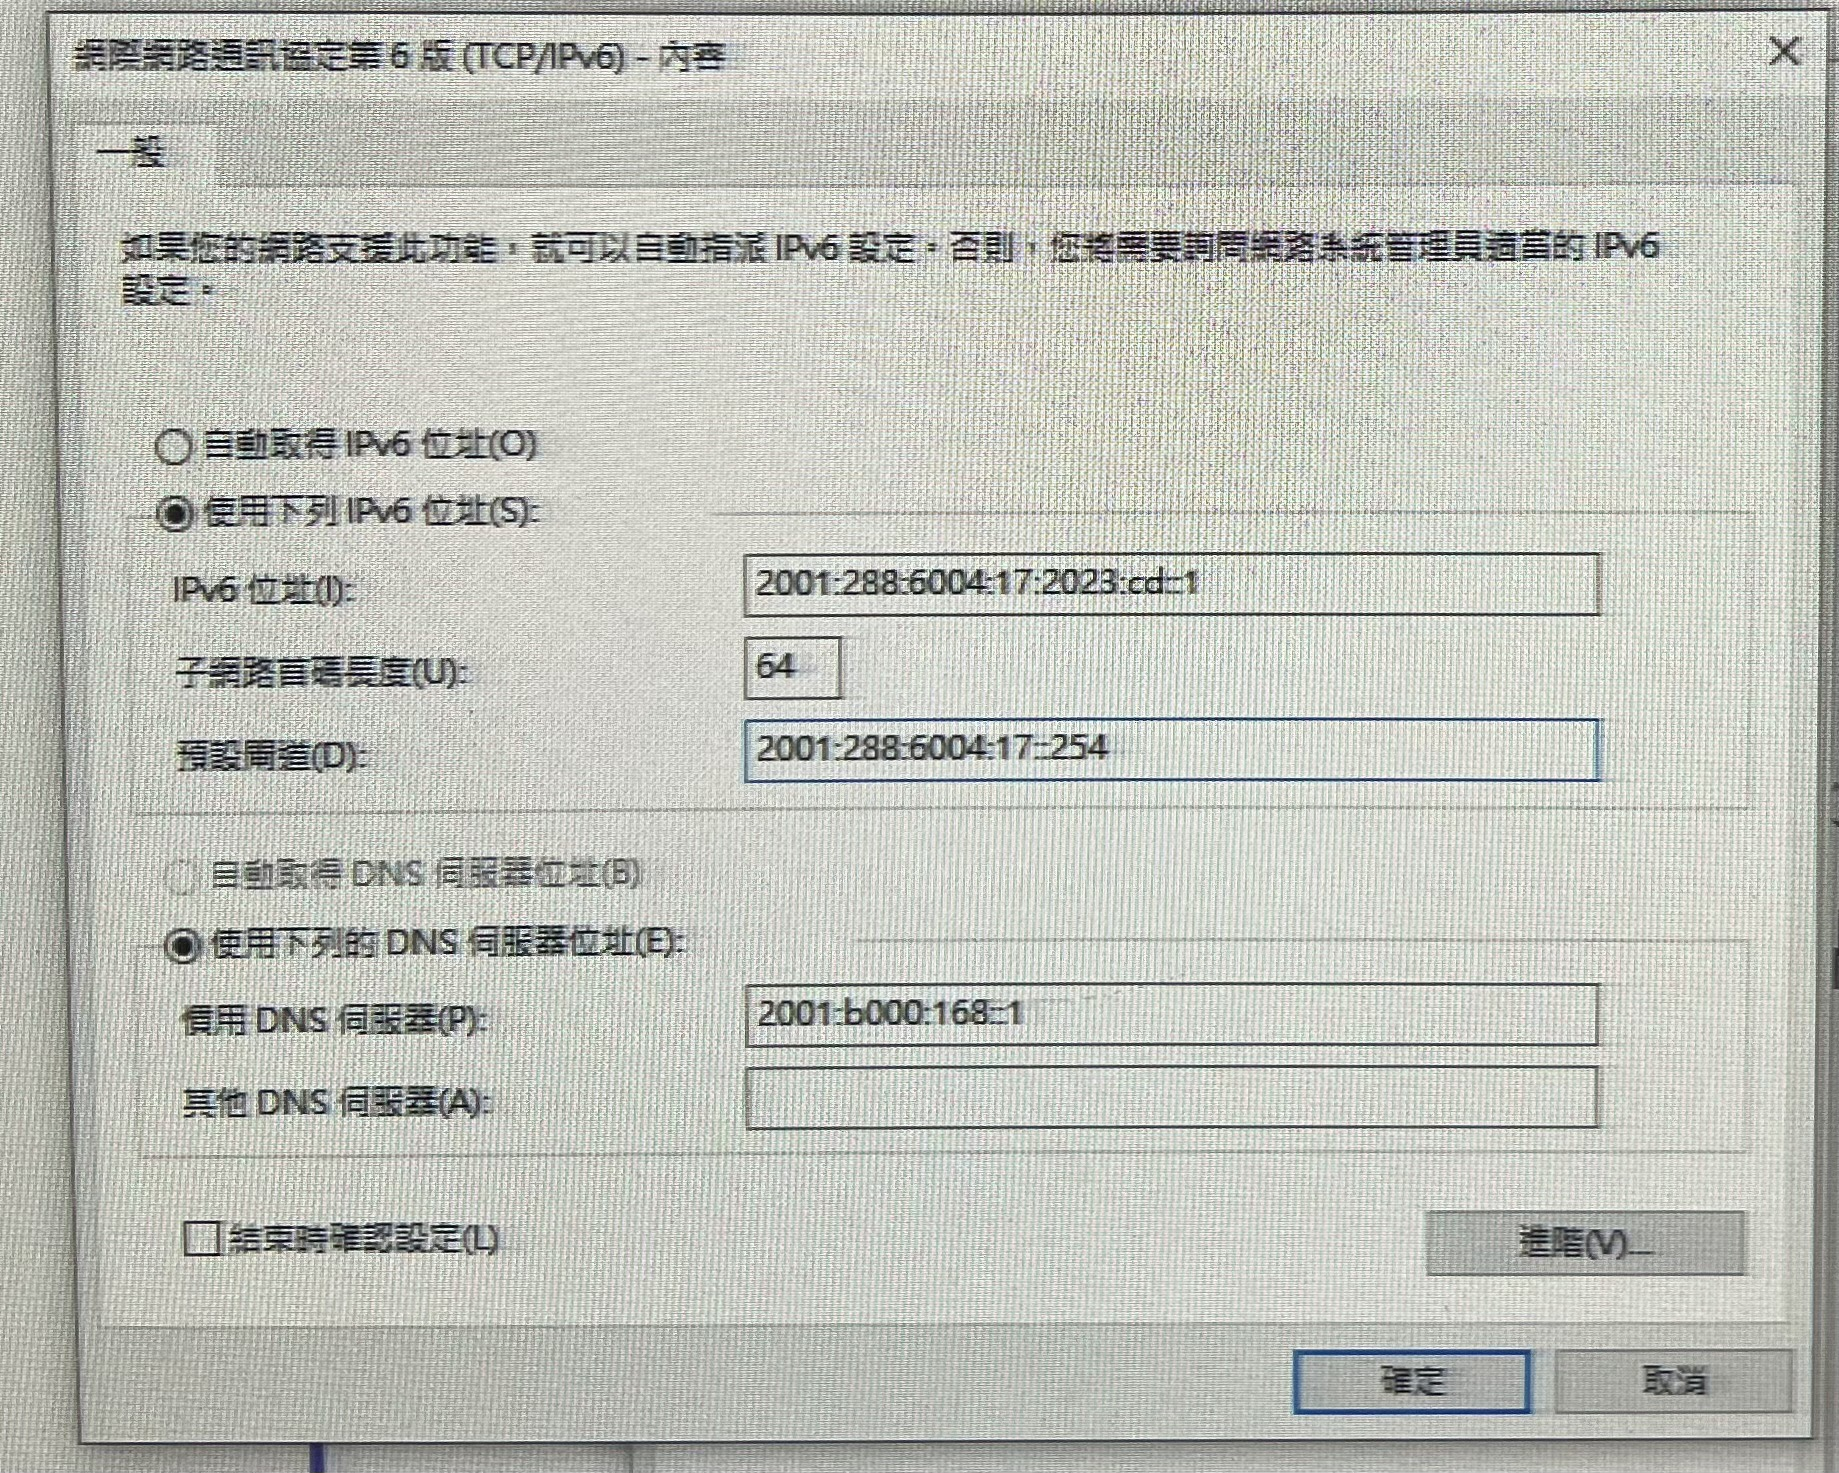
\includegraphics[width=10cm]{程式碼3}
\caption{\Large IPv6設置}\label{fig.程式碼3}
\end{center}
\end{figure}
\newpage

\begin{center}
到防火牆進階設定裡面,新增規則,然後將規則類型改成連接埠
\end{center}

\begin{figure}[hbt!]
\begin{center}
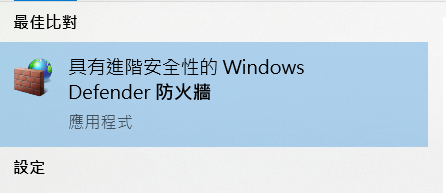
\includegraphics[width=10cm]{防火牆}
\caption{\Large 防火牆}\label{fig.防火牆}
\end{center}
\end{figure}

\begin{center}
將特定本機連接埠輸入23000至23050
\end{center}

\begin{figure}[hbt!]
\begin{center}
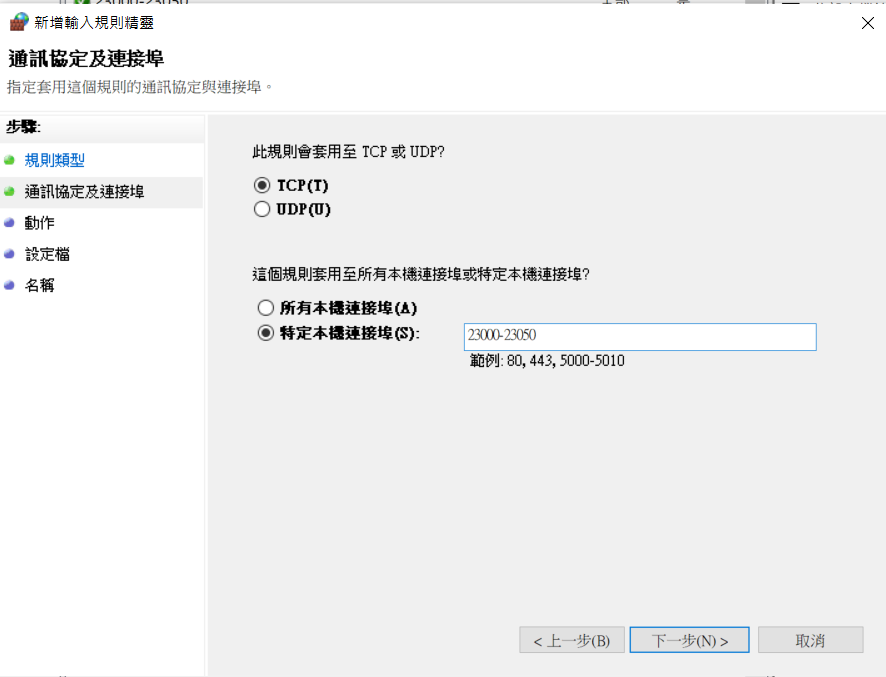
\includegraphics[width=10cm]{連接埠}
\caption{\Large 特定本機連接埠}\label{fig.連接埠}
\end{center}
\end{figure}

\begin{center}
下兩步為預設,到了名稱這裡打23000-23050
\end{center}

\begin{figure}[hbt!]
\begin{center}
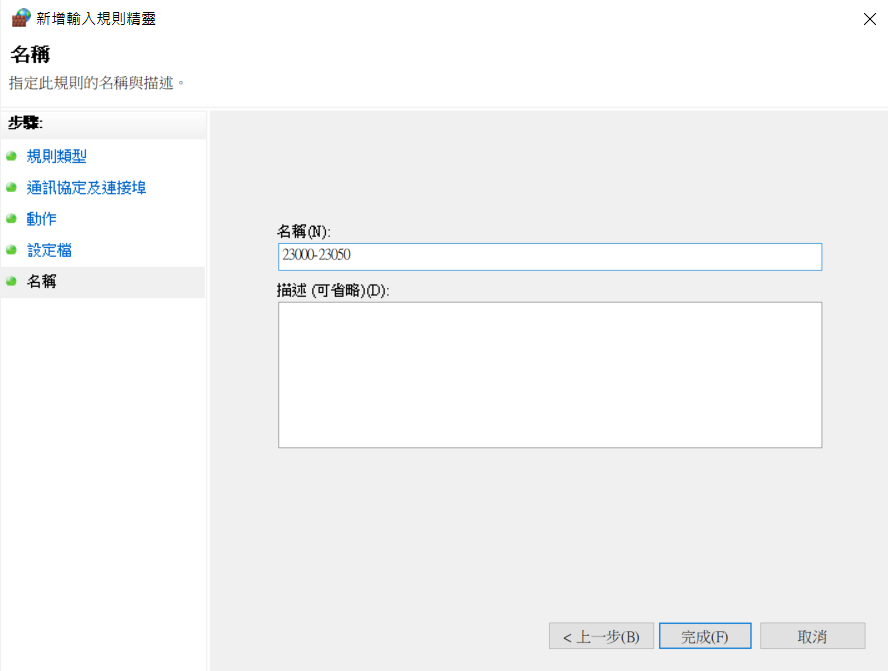
\includegraphics[width=10cm]{連接埠名稱}
\caption{\Large 連接埠名稱}\label{fig.連接埠名稱}
\end{center}
\end{figure}
\newpage


\begin{figure}[hbt!]
\begin{center}
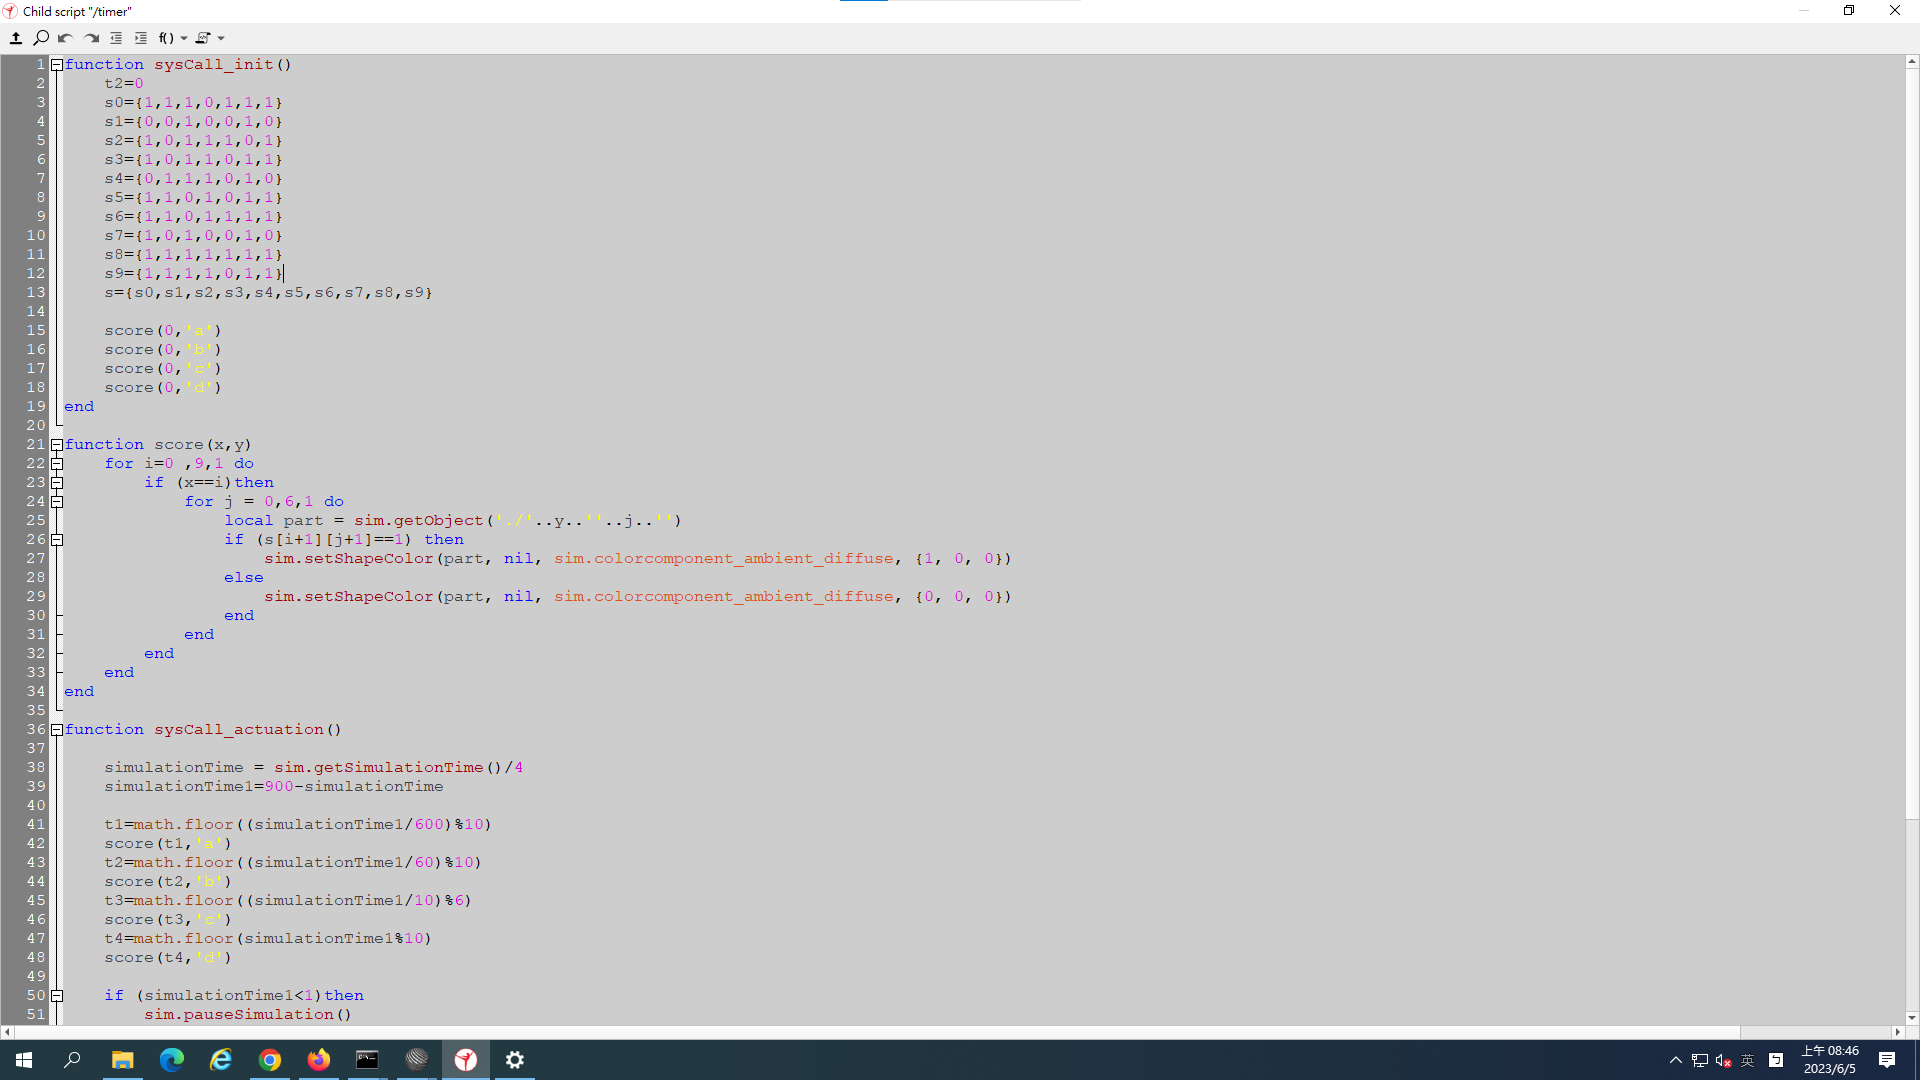
\includegraphics[width=20cm]{記分板程式碼}
\caption{\Large 記分板的程式碼}\label{fig.記分板程式碼}
\end{center}
\end{figure}
\newpage